\begin{frame}
	\frametitle{Procedimento 01}
	\framesubtitle{Desempenho}
	\only<1>{
		\begin{itemize}
			\item Em se tratando das bandas críticas, se verificou que BARK apresentou melhor desempenho em quase todas as combinações testadas.
			\item A combinação \textbf{\textit{wavelet} + Bark} apresentou, em geral, \textbf{melhor} viabilidade do que as respectivas combinações \textbf{\textit{wavelet + Mel}}.
			\item De todas as possibilidades verificadas a \textbf{\textit{wavelet} haar + Bark} apresentou o melhor desempenho.
		\end{itemize}
		
		\begin{center}
	\newcommand{\mc}[3]{\multicolumn{#1}{#2}{#3}}
	\definecolor{tcB}{rgb}{0.447059,0.74902,0.266667}
	\definecolor{tcA}{rgb}{0.65098,0.65098,0.65098}
	\definecolor{tcC}{rgb}{0,0.8,1}
	
	\begin{longtable}[h]{|c|c|c|c|c|}
		
		% Columns headers
		\hline
		\mc{1}{|>{\columncolor{tcA}}c|}{Mel/Bark}&\mc{1}{|>{\columncolor{tcA}}c|}{Wavelet}&\mc{1}{|>{\columncolor{tcA}}c|}{G1}&\mc{1}{|>{\columncolor{tcA}}c|}{G2}&\mc{1}{|>{\columncolor{tcA}}c|}{Distância de (1,0)}\\\hline
		\endfirsthead
		
		\mc{3}{c}{{\tablename\ \thetable : Continuação da página anterior}} \\\hline
		% Columns headers
		\mc{1}{|>{\columncolor{tcA}}c|}{Mel/Bark}&\mc{1}{|>{\columncolor{tcA}}c|}{Wavelet}&\mc{1}{|>{\columncolor{tcA}}c|}{G1}&\mc{1}{|>{\columncolor{tcA}}c|}{G2}&\mc{1}{|>{\columncolor{tcA}}c|}{Distance to (1,0)}\\\hline
		\endhead
		
		\hline \mc{2}{c}{{Continua na próxima página}} \\
		\endfoot
		\endlastfoot
		
		% Color of the first line
		\rowcolor{tcB}
		
		% Loads data from tables/results/paraconsistentPlane/distParacomFrom10.csv
		\csvreader[
		no head,
		late after line=\\\hline\rowcolor{tcC},%
		separator=comma,
		filter={\value{csvrow}<4},
		]{../monography/tables/results/paraconsistentPlane/distParacomFrom10.csv}{
			1=\melBark,
			2=\wavelet,
			3=\gOne,
			4=\gTwo,
			5=\distance
		}{
			\melBark&
			\wavelet&
			\StrSubstitute[0]{\gOne}{.}{,}&
			\StrSubstitute[0]{\gTwo}{.}{,}&
			\StrSubstitute[0]{\distance}{.}{,}
		}
		
		\rowcolor{white}
		\caption{As 5 primeiras combinações Wavelet \textit{x} Mel/Bark ordenadas pela distância do vértice (1,0) no plano paraconsistente.}
		\label{tab:distParacomFrom10BarkAndMel}
	\end{longtable}
\end{center}

	}
	\only<2>{
		\begin{textblock*}{\linewidth}(0.5cm,1.2cm)
			\begin{figure}[H]
				\centering
				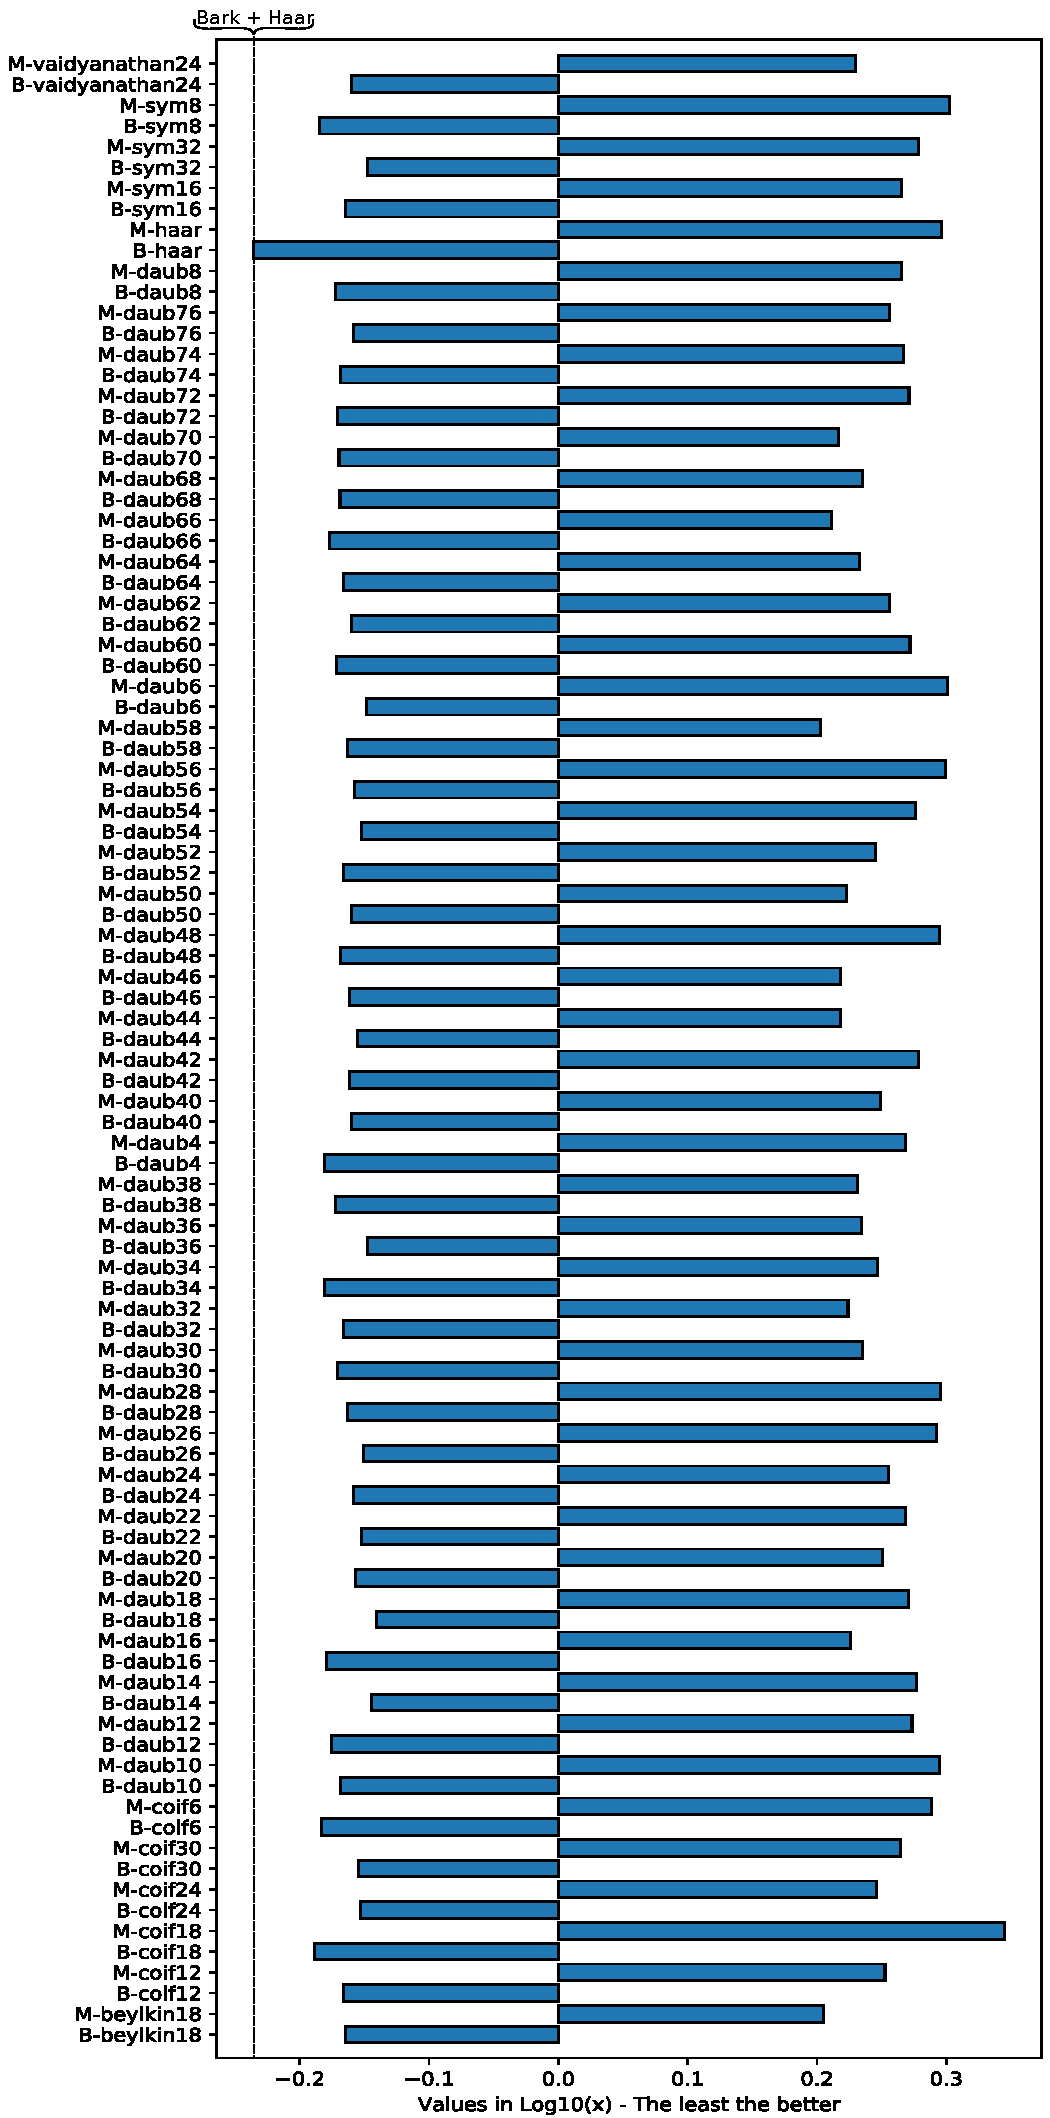
\includegraphics[width=5.6cm,angle=-90]{../monography/images/results/paraconsistentPlane/ParaconsistentFull.pdf}
				\caption{Distâncias de P=(G1, G2) ao ponto (1, 0) no plano paraconsistente. M=Mel; B=Bark; Sym=Symlet; Daub=Daubechies; Coif=Coiflet. Para uma melhor visualização, Uma unidade foi somada a cada distância e, a seguir, foi aplicado o $log_{10}$ no resultado correspondente.}
			\end{figure}
		\end{textblock*}
	}
	
	\only<3>{		
		\begin{figure}[H]
			\centering
			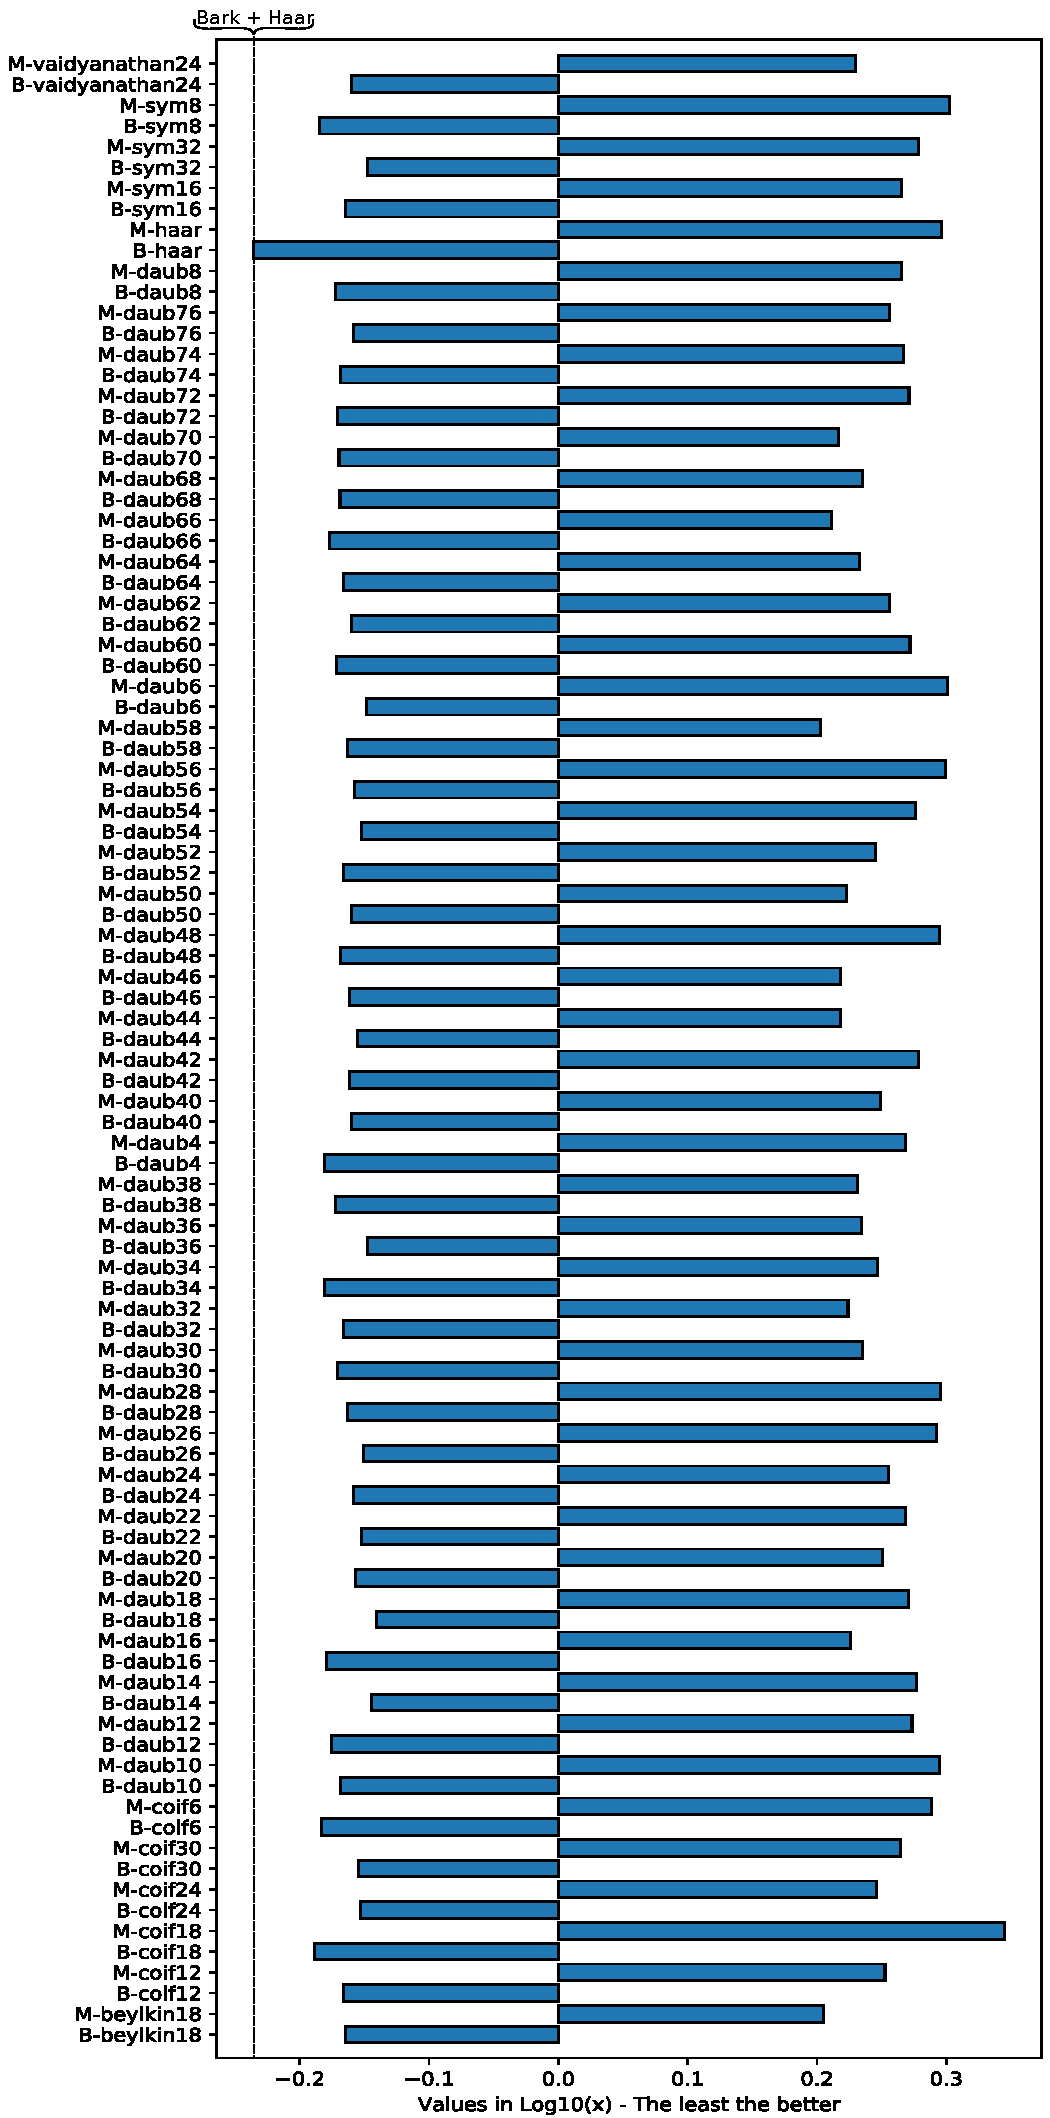
\includegraphics[width=5cm,angle=-90,trim=37 0 250 375,clip]{../monography/images/results/paraconsistentPlane/ParaconsistentFull.pdf}
			\caption{Detalhe: Combinação Bark + Wavelet Haar}
		\end{figure}
	}
	
	\only<4>{
		\framesubtitle{Síntese}
		\begin{columns}
			\column{0.5\textwidth}
			\begin{itemize}
				\item \textbf{Haar} e \textbf{Daubechies 76} proporcionaram, respectivamente, os melhores e os piores resultados associados com a escala Bark.
				\item Com a escala \textit{Mel}, \textbf{Haar} foi o melhor filtro e \textbf{Daubechies 8} o pior.
			\end{itemize}
			
			\par \textbf{\textit{Wavelet} Haar}
			\begin{itemize}
				\item Filtro de ordem 1
				\item Resposta perfeitamente linear.
				\item Contaminação por bandas adjacentes.
				\item Curva de resposta em frequência mais distante da ideal.
			\end{itemize}
			
			\column{0.5\textwidth}
			\par Portanto, experimentalmente, constatou-se que uma resposta em frequência não-rigorosa associada à uma resposta em fase perfeitamente linear é a melhor alternativa.\newline
			
			\par A \textbf{característica ruidosa} dos sinais regravados, contendo, ao contrário das vozes originais, notórios componentes de altas frequências, é melhor detectada com uma escala mais apropriada ao tratamento de áudio em geral e não voz somente.	
		\end{columns}
	}
	
\end{frame}